\documentclass[tikz,convert={outfile=images/liftFree-nat.svg,density=1000}]{standalone}
\usepackage[build={latexoptions={-output-directory=latex/svg}}]{standalone}
\begin{document}
\tikzstyle{every node}=[font=\footnotesize]
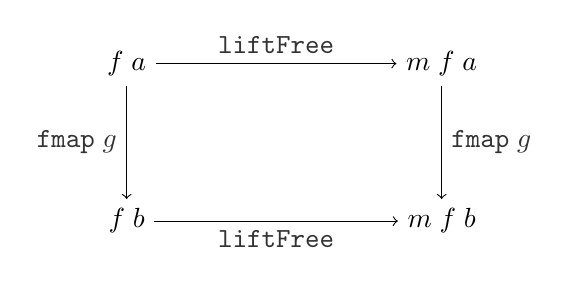
\begin{tikzpicture}
    \node (A) at (0,2) {\texttt{$f\;a$}};
    \node (B) at (4,2) {\texttt{$m\;f\;a$}};
    \node (C) at (0,0) {\texttt{$f\;b$}};
    \node (D) at (4,0) {\texttt{$m\;f\;b$}};
    \draw[->] (A) -- node[left] {\textcolor{black!80}{$\texttt{fmap}\;g$}} (C);
    \draw[->] (B) -- node[right] {\textcolor{black!80}{$\texttt{fmap}\;g$}} (D);
    \draw[->] (A) -- node [above] {\textcolor{black!80}{$\texttt{liftFree}$}} (B);
    \draw[->] (C) -- node [below] {\textcolor{black!80}{$\texttt{liftFree}$}} (D);
\end{tikzpicture}
\end{document}
